\section{Results}
\label{sec:results}

\subsection{Compactness Measures}
\begin{figure}[h]
    \caption{Distributions of Compactness Measures for \hyperref[sec:smc]{SMC}- and \hyperref[sec:crsg]{CRSG}-Generated Maps}
    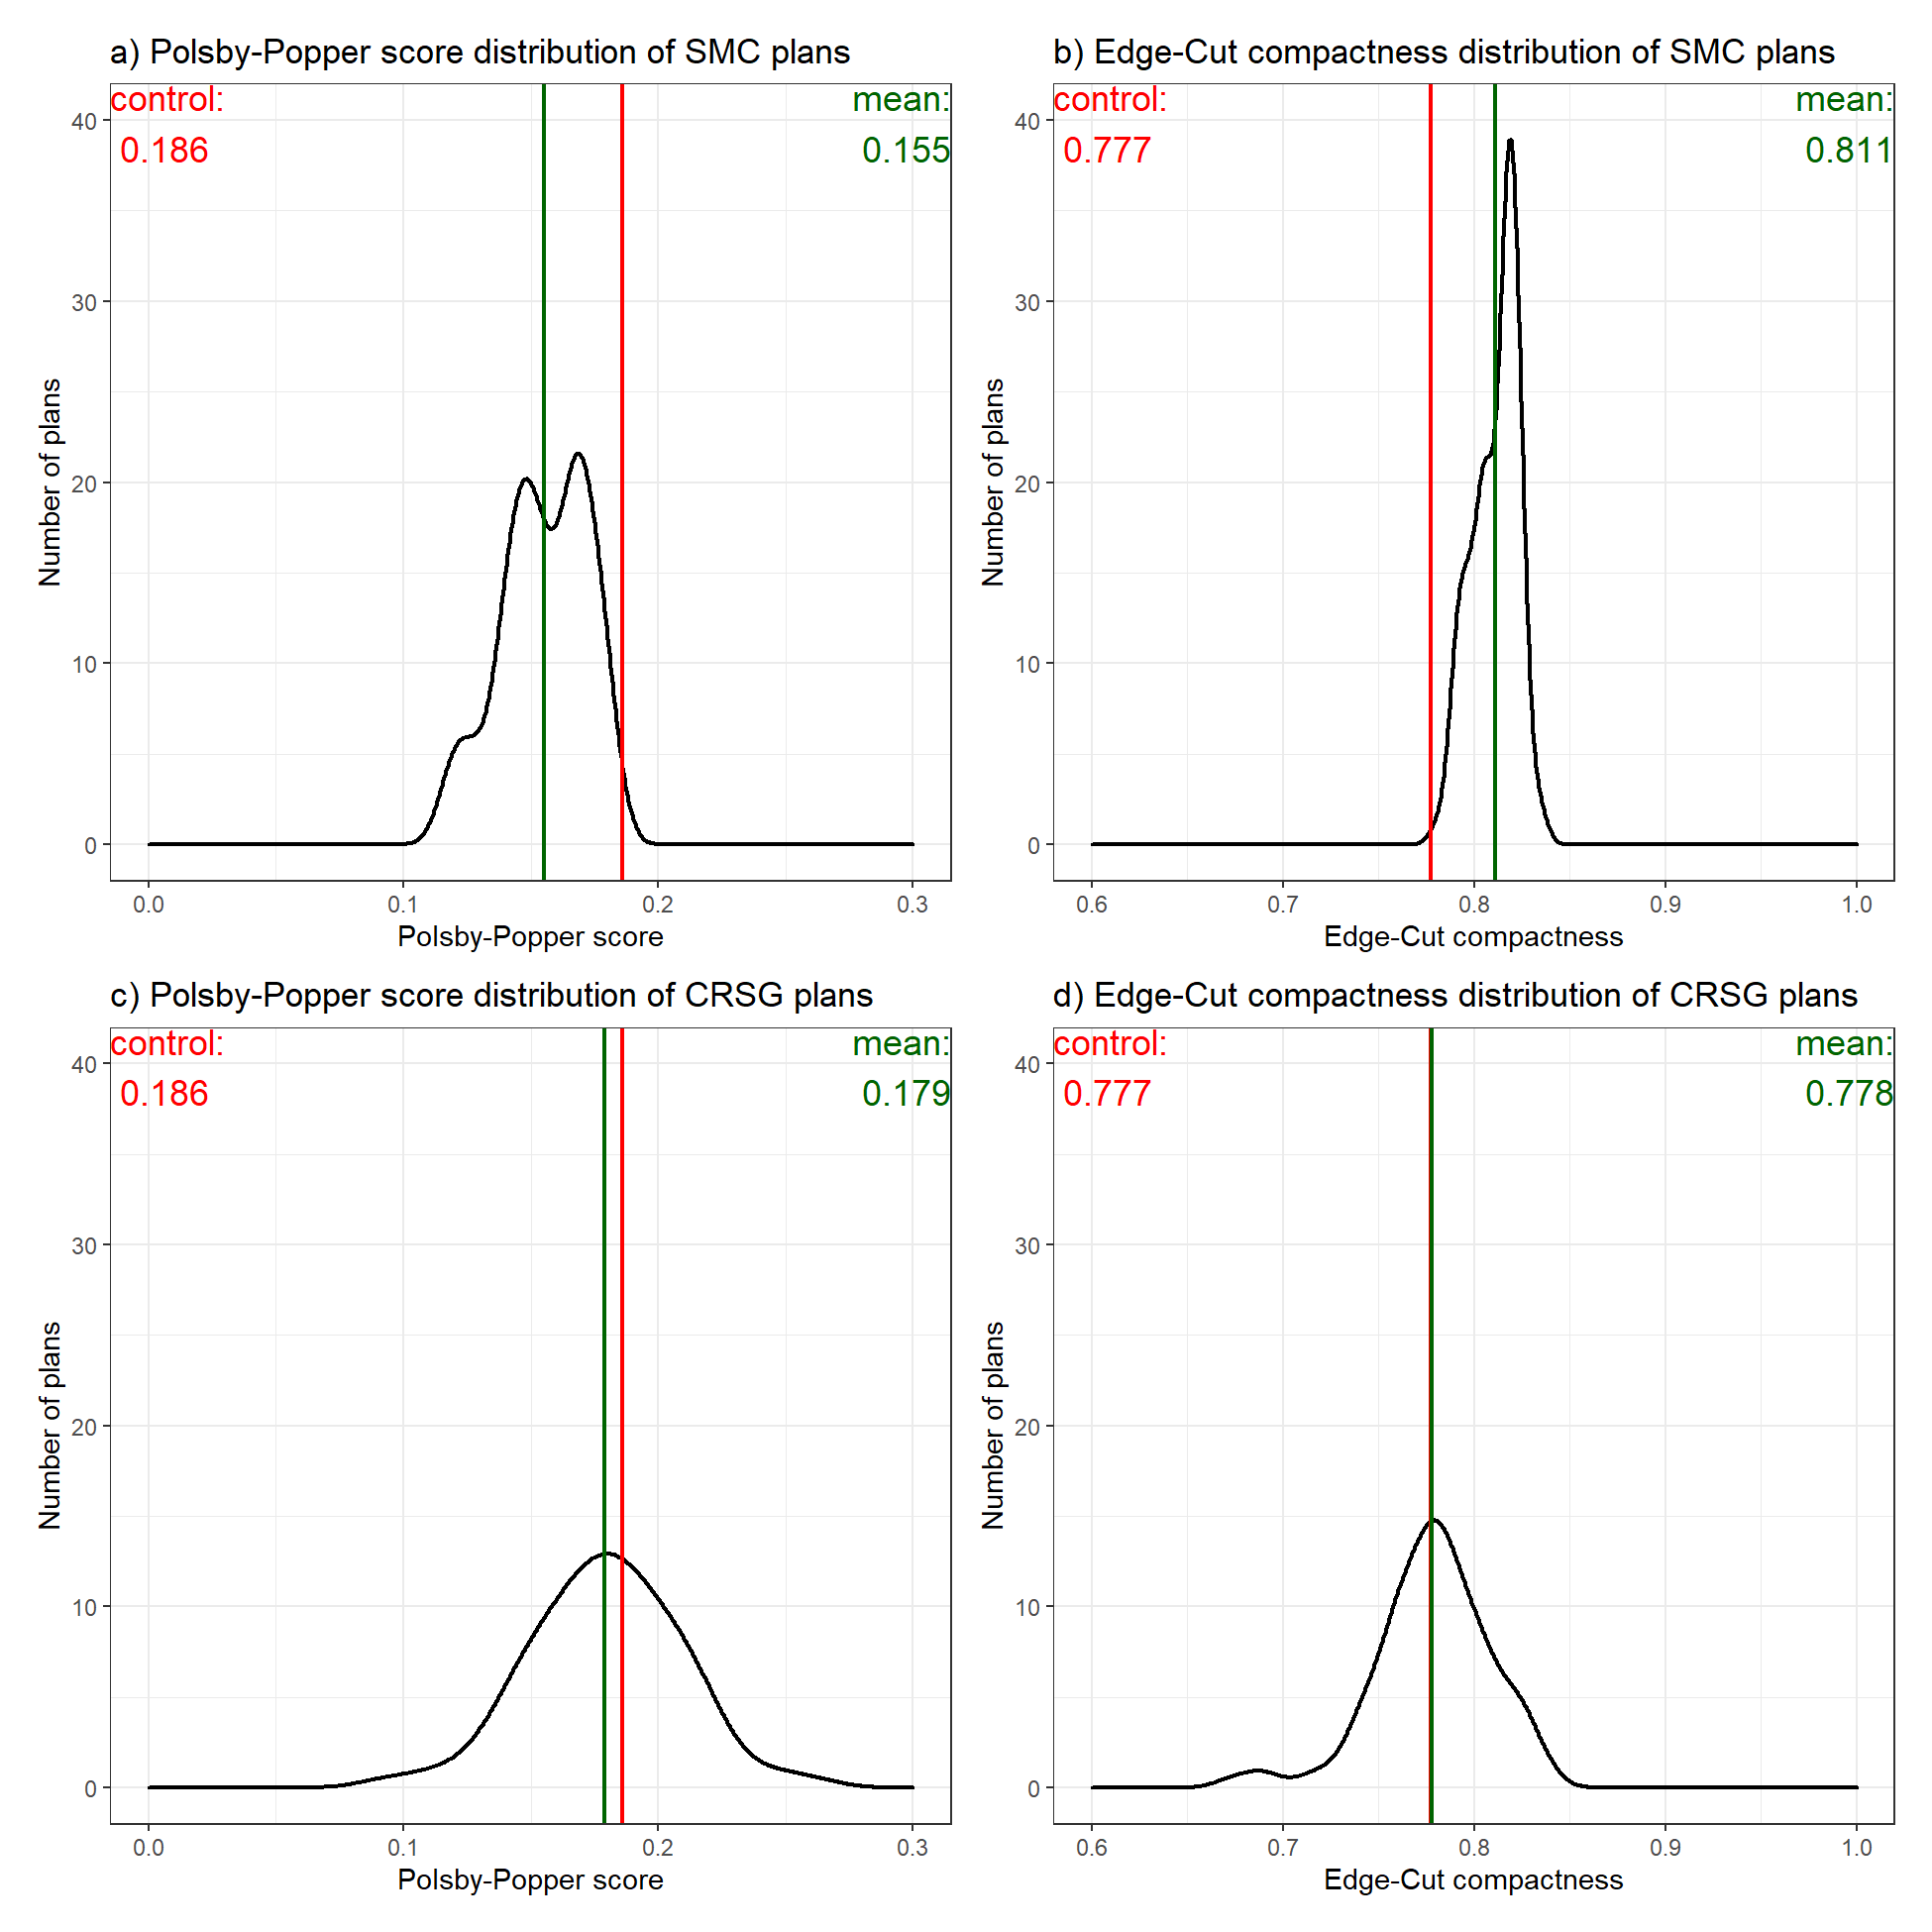
\includegraphics[width=\textwidth]{img/compact.density.png}
    \label{fig:compact.density}
    \raggedright
    \figurenote{The first column of plots shows the \hyperref[sec:polsbypopper]{Polsby-Popper} score distribution; the second column shows the \hyperref[sec:edgecut]{edge-cut compactness measure} distribution. The first row corresponds to the maps generated by \hyperref[sec:smc]{SMC}; the second row corresponds to \hyperref[sec:crsg]{CRSG}. The dashed red lines indicate the measure value for the existing districts; the solid blue lines indicate the mean value of the distribution.}
\end{figure}

Figure \ref{fig:compact.density} visualizes the distribution of two different compactness scores amongst maps generated by both SMC and CRSG. Subfigure
\begin{seriate} 
    \item shows the distribution of the \hyperref[sec:polsbypopper]{Polsby-Popper score} of the 100 SMC maps, subfigure
    \item shows the distribution of the \hyperref[sec:edgecut]{edge-cut compactness measure} of the same 100 SMC maps, and subfigures
    \item and 
    \item show the corresponding measure distributions for the maps generated by CRSG. 
\end{seriate}
The dashed red lines indicate the value of the measure for the existing district map, and the solid blue lines indicate the mean value of the distribution. 

\subsection{Partisan Fairness}

\subsubsection{Seats-Votes Curves}

\begin{figure}[h]
    \caption{\hyperref[sec:seatsvotes]{Seats-Votes Curves} for \hyperref[sec:smc]{SMC}- and \hyperref[sec:crsg]{CRSG}-Generated Maps and Existing Map}
    \begin{subfigure}[b]{0.45\textwidth}
        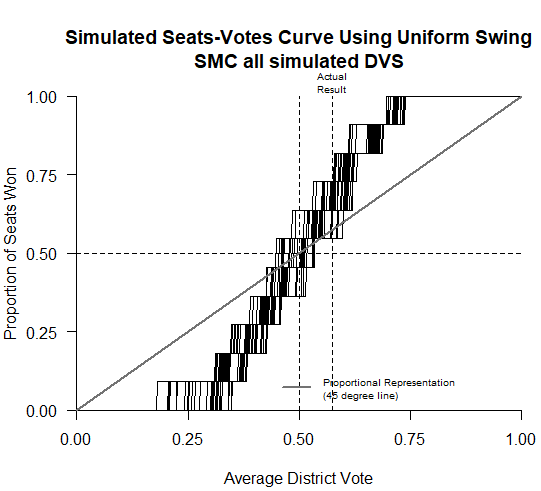
\includegraphics[width=\textwidth]{img/sv.smc.png}
        \caption{SMC Seats-Votes Curve}
        \label{fig:sv.smc}
    \end{subfigure}
    \hfill
    \begin{subfigure}[b]{0.45\textwidth}
        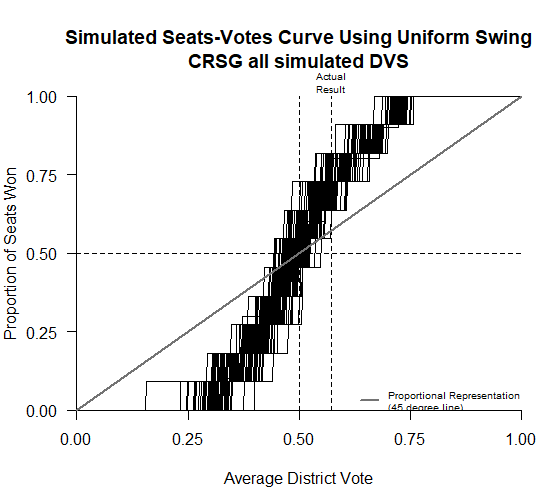
\includegraphics[width=\textwidth]{img/sv.crsg.png}
        \caption{CRSG Seats-Votes Curve}
        \label{fig:sv.crsg}
    \end{subfigure}
    \vskip\baselineskip
    %\hfill
    \begin{subfigure}[b]{0.45\textwidth}
        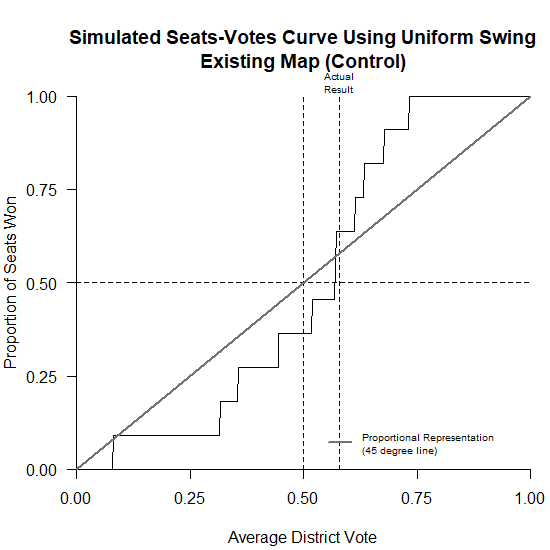
\includegraphics[width=\textwidth]{img/sv.control.png}
        \caption{Control Seats-Votes Curve}
        \label{fig:sv.control}
    \end{subfigure}
    \label{fig:sv}
    \raggedright
    \figurenote{Each plot shows the relationship between the average proportion of votes won by Democrats in each district and the proportion seats in the delegation won by Democrats. Subfigure \ref{fig:sv.smc} illustrates this relationship for the 100 maps generated by SMC, subfigure \ref{fig:sv.crsg} for CRSG, and subfigure \ref{fig:sv.control} is for the existing map.}
\end{figure}

Figure \ref{fig:sv} shows the \hyperref[sec:seatsvotes]{seats-votes curves} \parencite{katz2020} for the 2018 General Election under the redistricting maps generated by both algorithms and the existing map, the control. For each plot, the x-axis plots the average of the proportion of votes won by Democrats in each district (DVS). The y-axis plots the proportion of seats won by Democrats in the delegation. Both subfigures \ref{fig:sv.smc} and \ref{fig:sv.crsg} have once curve for each redistricting map (each plot has 100 curves). The seats-votes curve for the existing 2018 districts is provided for reference in subfigure \ref{fig:sv.control}.

\subsubsection{Single-Valued Partisan Fairness Measures}

Figure \ref{fig:fair.density} illustrates the distributions of various partisan fairness measures computed for the maps generated by SMC and CRSG. Columns of plots correspond to different measures, and rows of plots correspond to different algorithms. The dashed red and solid blue vertical lines indicate the control values and mean distribution values, respectively. 

\begin{landscape}
    \begin{figure}[h]
        \caption{Distributions of Partisan Fairness Measures for \hyperref[sec:smc]{SMC}- and \hyperref[sec:crsg]{CRSG}-Generated Maps}
        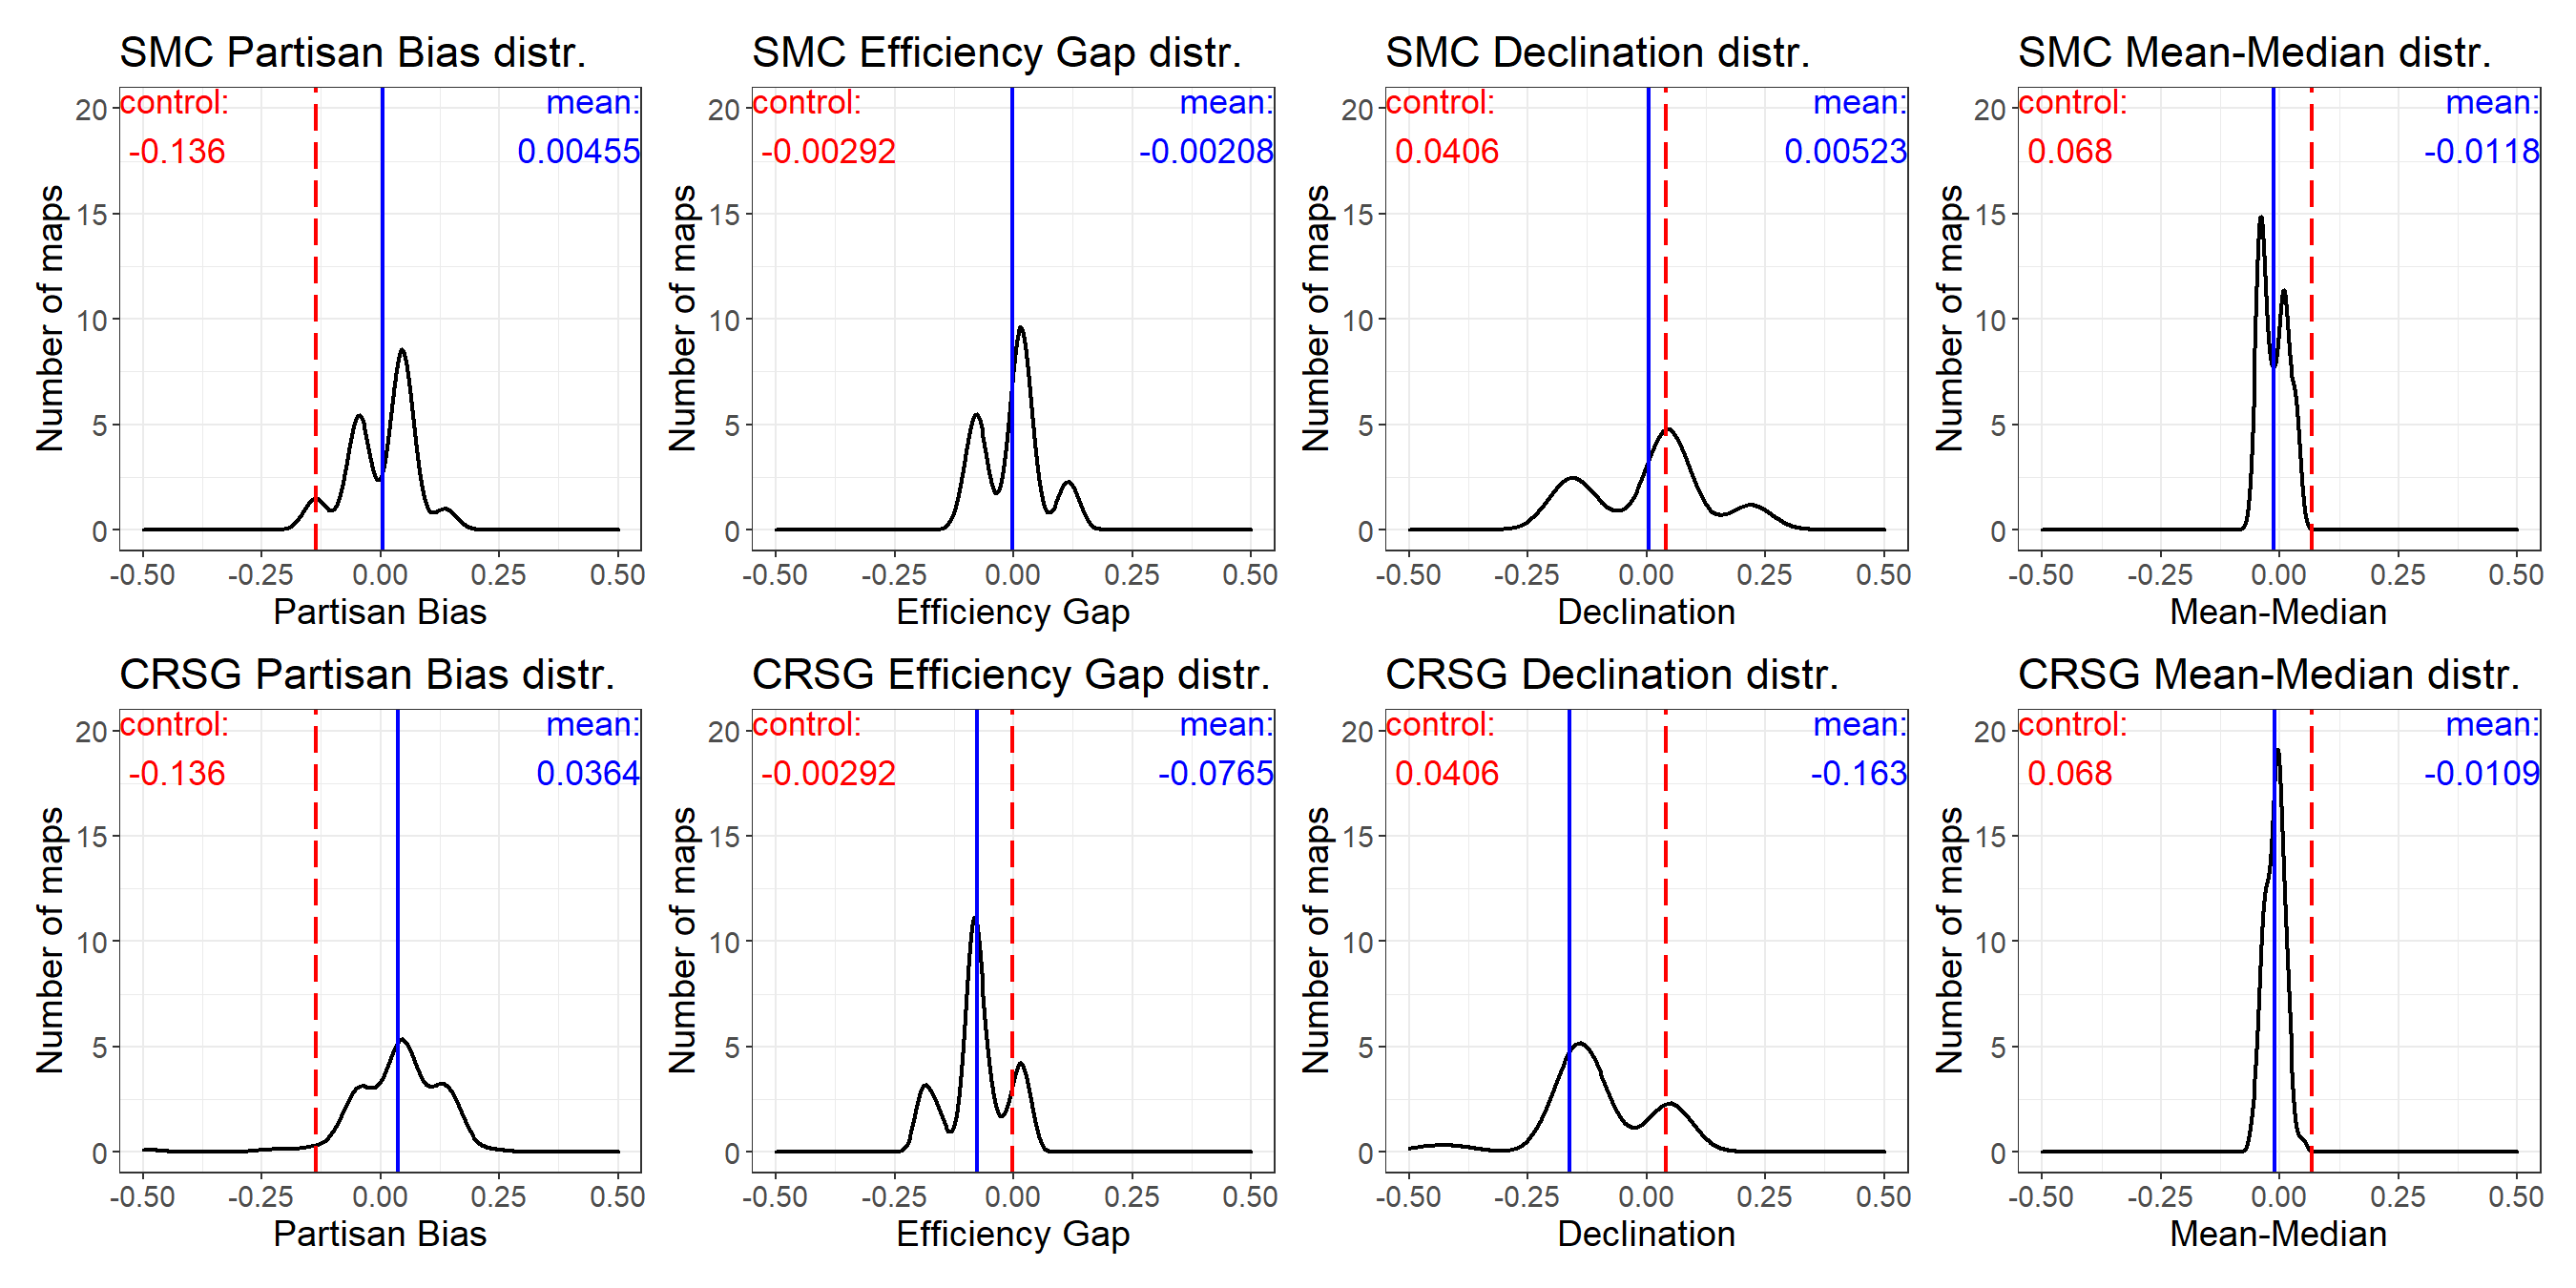
\includegraphics{img/fair.density.png}
        \label{fig:fair.density}
        \raggedright
        \figurenote{From left to right, the columns of plots illustrate the distributions of \hyperref[sec:bias]{partisan bias}, the \hyperref[sec:effgap]{efficiency gap}, \hyperref[sec:declination]{declination}, and the \hyperref[sec:meanmed]{mean-median difference}, respectively. The first row of plots corresponds to SMC maps, the second to CRSG maps. The dashed red lines indicate the corresponding value of the measure computed for the existing map; the solid blue lines indicate the mean values of the distributions.}
    \end{figure}
\end{landscape}